% Created by tikzDevice version 0.12.6 on 2024-08-04 19:03:26
% !TEX encoding = UTF-8 Unicode
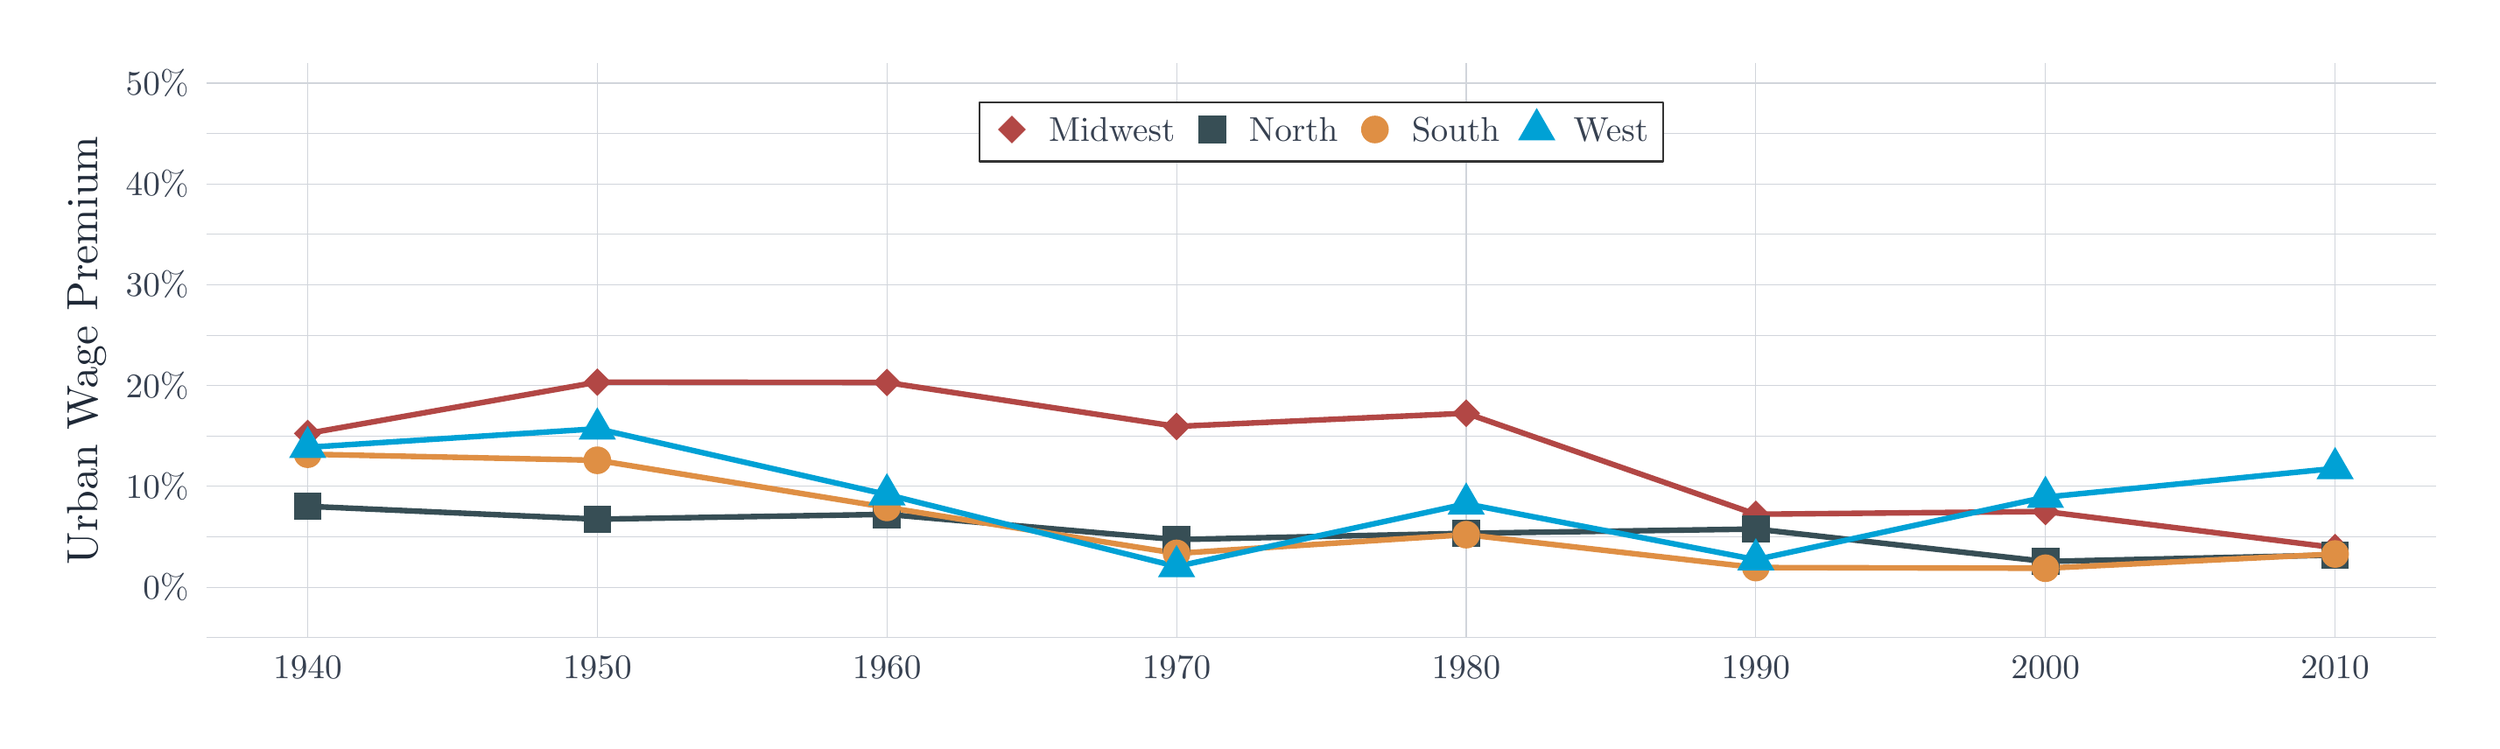
\begin{tikzpicture}[x=1pt,y=1pt]
\definecolor{fillColor}{RGB}{255,255,255}
\path[use as bounding box,fill=fillColor] (0,0) rectangle (1011.78,289.08);
\begin{scope}
\path[clip] (  0.00,  0.00) rectangle (1011.78,289.08);
\definecolor{drawColor}{RGB}{255,255,255}

\path[draw=drawColor,line width= 0.8pt,line join=round,line cap=round,fill=fillColor] (  0.00,  0.00) rectangle (1011.78,289.08);
\end{scope}
\begin{scope}
\path[clip] ( 75.16, 35.76) rectangle (995.78,273.08);
\definecolor{drawColor}{RGB}{255,255,255}
\definecolor{fillColor}{RGB}{255,255,255}

\path[draw=drawColor,line width= 0.8pt,line join=round,line cap=round,fill=fillColor] ( 75.16, 35.76) rectangle (995.78,273.08);
\definecolor{drawColor}{RGB}{209,213,219}

\path[draw=drawColor,line width= 0.4pt,line join=round] ( 75.16, 35.76) --
	(995.78, 35.76);

\path[draw=drawColor,line width= 0.4pt,line join=round] ( 75.16, 77.39) --
	(995.78, 77.39);

\path[draw=drawColor,line width= 0.4pt,line join=round] ( 75.16,119.03) --
	(995.78,119.03);

\path[draw=drawColor,line width= 0.4pt,line join=round] ( 75.16,160.66) --
	(995.78,160.66);

\path[draw=drawColor,line width= 0.4pt,line join=round] ( 75.16,202.30) --
	(995.78,202.30);

\path[draw=drawColor,line width= 0.4pt,line join=round] ( 75.16,243.94) --
	(995.78,243.94);

\path[draw=drawColor,line width= 0.4pt,line join=round] ( 75.16, 56.58) --
	(995.78, 56.58);

\path[draw=drawColor,line width= 0.4pt,line join=round] ( 75.16, 98.21) --
	(995.78, 98.21);

\path[draw=drawColor,line width= 0.4pt,line join=round] ( 75.16,139.85) --
	(995.78,139.85);

\path[draw=drawColor,line width= 0.4pt,line join=round] ( 75.16,181.48) --
	(995.78,181.48);

\path[draw=drawColor,line width= 0.4pt,line join=round] ( 75.16,223.12) --
	(995.78,223.12);

\path[draw=drawColor,line width= 0.4pt,line join=round] ( 75.16,264.75) --
	(995.78,264.75);

\path[draw=drawColor,line width= 0.4pt,line join=round] (117.01, 35.76) --
	(117.01,273.08);

\path[draw=drawColor,line width= 0.4pt,line join=round] (236.57, 35.76) --
	(236.57,273.08);

\path[draw=drawColor,line width= 0.4pt,line join=round] (356.13, 35.76) --
	(356.13,273.08);

\path[draw=drawColor,line width= 0.4pt,line join=round] (475.69, 35.76) --
	(475.69,273.08);

\path[draw=drawColor,line width= 0.4pt,line join=round] (595.25, 35.76) --
	(595.25,273.08);

\path[draw=drawColor,line width= 0.4pt,line join=round] (714.81, 35.76) --
	(714.81,273.08);

\path[draw=drawColor,line width= 0.4pt,line join=round] (834.37, 35.76) --
	(834.37,273.08);

\path[draw=drawColor,line width= 0.4pt,line join=round] (953.93, 35.76) --
	(953.93,273.08);
\definecolor{drawColor}{RGB}{178,71,69}

\path[draw=drawColor,line width= 2.3pt,line join=round] (117.01,120.08) --
	(236.57,141.27) --
	(356.13,141.12) --
	(475.69,122.98) --
	(595.25,128.42) --
	(714.81, 86.71) --
	(834.37, 87.83) --
	(953.93, 72.92);
\definecolor{drawColor}{RGB}{55,78,85}

\path[draw=drawColor,line width= 2.3pt,line join=round] (117.01, 89.99) --
	(236.57, 84.67) --
	(356.13, 86.66) --
	(475.69, 76.25) --
	(595.25, 78.84) --
	(714.81, 80.60) --
	(834.37, 67.21) --
	(953.93, 69.85);
\definecolor{drawColor}{RGB}{223,143,68}

\path[draw=drawColor,line width= 2.3pt,line join=round] (117.01,111.51) --
	(236.57,108.99) --
	(356.13, 89.53) --
	(475.69, 70.54) --
	(595.25, 78.28) --
	(714.81, 64.70) --
	(834.37, 64.41) --
	(953.93, 70.29);
\definecolor{drawColor}{RGB}{0,161,213}

\path[draw=drawColor,line width= 2.3pt,line join=round] (117.01,114.36) --
	(236.57,122.01) --
	(356.13, 94.83) --
	(475.69, 65.14) --
	(595.25, 91.01) --
	(714.81, 67.97) --
	(834.37, 93.77) --
	(953.93,105.64);
\definecolor{fillColor}{RGB}{178,71,69}

\path[fill=fillColor] (111.30,120.08) --
	(117.01,125.79) --
	(122.72,120.08) --
	(117.01,114.37) --
	cycle;
\definecolor{fillColor}{RGB}{55,78,85}

\path[fill=fillColor] (111.30, 84.28) --
	(122.72, 84.28) --
	(122.72, 95.70) --
	(111.30, 95.70) --
	cycle;
\definecolor{fillColor}{RGB}{223,143,68}

\path[fill=fillColor] (117.01,111.51) circle (  5.71);
\definecolor{fillColor}{RGB}{0,161,213}

\path[fill=fillColor] (117.01,123.24) --
	(124.70,109.92) --
	(109.32,109.92) --
	cycle;
\definecolor{fillColor}{RGB}{178,71,69}

\path[fill=fillColor] (230.86,141.27) --
	(236.57,146.98) --
	(242.28,141.27) --
	(236.57,135.56) --
	cycle;
\definecolor{fillColor}{RGB}{55,78,85}

\path[fill=fillColor] (230.86, 78.96) --
	(242.28, 78.96) --
	(242.28, 90.38) --
	(230.86, 90.38) --
	cycle;
\definecolor{fillColor}{RGB}{223,143,68}

\path[fill=fillColor] (236.57,108.99) circle (  5.71);
\definecolor{fillColor}{RGB}{0,161,213}

\path[fill=fillColor] (236.57,130.89) --
	(244.26,117.57) --
	(228.88,117.57) --
	cycle;
\definecolor{fillColor}{RGB}{178,71,69}

\path[fill=fillColor] (350.42,141.12) --
	(356.13,146.83) --
	(361.84,141.12) --
	(356.13,135.41) --
	cycle;
\definecolor{fillColor}{RGB}{55,78,85}

\path[fill=fillColor] (350.42, 80.95) --
	(361.84, 80.95) --
	(361.84, 92.37) --
	(350.42, 92.37) --
	cycle;
\definecolor{fillColor}{RGB}{223,143,68}

\path[fill=fillColor] (356.13, 89.53) circle (  5.71);
\definecolor{fillColor}{RGB}{0,161,213}

\path[fill=fillColor] (356.13,103.71) --
	(363.82, 90.39) --
	(348.44, 90.39) --
	cycle;
\definecolor{fillColor}{RGB}{178,71,69}

\path[fill=fillColor] (469.98,122.98) --
	(475.69,128.69) --
	(481.40,122.98) --
	(475.69,117.27) --
	cycle;
\definecolor{fillColor}{RGB}{55,78,85}

\path[fill=fillColor] (469.98, 70.54) --
	(481.40, 70.54) --
	(481.40, 81.96) --
	(469.98, 81.96) --
	cycle;
\definecolor{fillColor}{RGB}{223,143,68}

\path[fill=fillColor] (475.69, 70.54) circle (  5.71);
\definecolor{fillColor}{RGB}{0,161,213}

\path[fill=fillColor] (475.69, 74.02) --
	(483.38, 60.70) --
	(468.00, 60.70) --
	cycle;
\definecolor{fillColor}{RGB}{178,71,69}

\path[fill=fillColor] (589.54,128.42) --
	(595.25,134.13) --
	(600.96,128.42) --
	(595.25,122.71) --
	cycle;
\definecolor{fillColor}{RGB}{55,78,85}

\path[fill=fillColor] (589.54, 73.13) --
	(600.96, 73.13) --
	(600.96, 84.55) --
	(589.54, 84.55) --
	cycle;
\definecolor{fillColor}{RGB}{223,143,68}

\path[fill=fillColor] (595.25, 78.28) circle (  5.71);
\definecolor{fillColor}{RGB}{0,161,213}

\path[fill=fillColor] (595.25, 99.89) --
	(602.94, 86.57) --
	(587.56, 86.57) --
	cycle;
\definecolor{fillColor}{RGB}{178,71,69}

\path[fill=fillColor] (709.10, 86.71) --
	(714.81, 92.42) --
	(720.52, 86.71) --
	(714.81, 81.00) --
	cycle;
\definecolor{fillColor}{RGB}{55,78,85}

\path[fill=fillColor] (709.10, 74.89) --
	(720.52, 74.89) --
	(720.52, 86.31) --
	(709.10, 86.31) --
	cycle;
\definecolor{fillColor}{RGB}{223,143,68}

\path[fill=fillColor] (714.81, 64.70) circle (  5.71);
\definecolor{fillColor}{RGB}{0,161,213}

\path[fill=fillColor] (714.81, 76.85) --
	(722.50, 63.53) --
	(707.12, 63.53) --
	cycle;
\definecolor{fillColor}{RGB}{178,71,69}

\path[fill=fillColor] (828.66, 87.83) --
	(834.37, 93.54) --
	(840.08, 87.83) --
	(834.37, 82.12) --
	cycle;
\definecolor{fillColor}{RGB}{55,78,85}

\path[fill=fillColor] (828.66, 61.50) --
	(840.08, 61.50) --
	(840.08, 72.92) --
	(828.66, 72.92) --
	cycle;
\definecolor{fillColor}{RGB}{223,143,68}

\path[fill=fillColor] (834.37, 64.41) circle (  5.71);
\definecolor{fillColor}{RGB}{0,161,213}

\path[fill=fillColor] (834.37,102.65) --
	(842.06, 89.33) --
	(826.68, 89.33) --
	cycle;
\definecolor{fillColor}{RGB}{178,71,69}

\path[fill=fillColor] (948.22, 72.92) --
	(953.93, 78.63) --
	(959.64, 72.92) --
	(953.93, 67.20) --
	cycle;
\definecolor{fillColor}{RGB}{55,78,85}

\path[fill=fillColor] (948.22, 64.14) --
	(959.64, 64.14) --
	(959.64, 75.56) --
	(948.22, 75.56) --
	cycle;
\definecolor{fillColor}{RGB}{223,143,68}

\path[fill=fillColor] (953.93, 70.29) circle (  5.71);
\definecolor{fillColor}{RGB}{0,161,213}

\path[fill=fillColor] (953.93,114.52) --
	(961.62,101.20) --
	(946.24,101.20) --
	cycle;
\end{scope}
\begin{scope}
\path[clip] (  0.00,  0.00) rectangle (1011.78,289.08);
\definecolor{drawColor}{RGB}{55,65,81}

\node[text=drawColor,anchor=base east,inner sep=0pt, outer sep=0pt, scale=  1.42] at ( 67.96, 51.68) {0\%};

\node[text=drawColor,anchor=base east,inner sep=0pt, outer sep=0pt, scale=  1.42] at ( 67.96, 93.31) {10\%};

\node[text=drawColor,anchor=base east,inner sep=0pt, outer sep=0pt, scale=  1.42] at ( 67.96,134.95) {20\%};

\node[text=drawColor,anchor=base east,inner sep=0pt, outer sep=0pt, scale=  1.42] at ( 67.96,176.59) {30\%};

\node[text=drawColor,anchor=base east,inner sep=0pt, outer sep=0pt, scale=  1.42] at ( 67.96,218.22) {40\%};

\node[text=drawColor,anchor=base east,inner sep=0pt, outer sep=0pt, scale=  1.42] at ( 67.96,259.86) {50\%};
\end{scope}
\begin{scope}
\path[clip] (  0.00,  0.00) rectangle (1011.78,289.08);
\definecolor{drawColor}{RGB}{55,65,81}

\node[text=drawColor,anchor=base,inner sep=0pt, outer sep=0pt, scale=  1.42] at (117.01, 18.76) {1940};

\node[text=drawColor,anchor=base,inner sep=0pt, outer sep=0pt, scale=  1.42] at (236.57, 18.76) {1950};

\node[text=drawColor,anchor=base,inner sep=0pt, outer sep=0pt, scale=  1.42] at (356.13, 18.76) {1960};

\node[text=drawColor,anchor=base,inner sep=0pt, outer sep=0pt, scale=  1.42] at (475.69, 18.76) {1970};

\node[text=drawColor,anchor=base,inner sep=0pt, outer sep=0pt, scale=  1.42] at (595.25, 18.76) {1980};

\node[text=drawColor,anchor=base,inner sep=0pt, outer sep=0pt, scale=  1.42] at (714.81, 18.76) {1990};

\node[text=drawColor,anchor=base,inner sep=0pt, outer sep=0pt, scale=  1.42] at (834.37, 18.76) {2000};

\node[text=drawColor,anchor=base,inner sep=0pt, outer sep=0pt, scale=  1.42] at (953.93, 18.76) {2010};
\end{scope}
\begin{scope}
\path[clip] (  0.00,  0.00) rectangle (1011.78,289.08);
\definecolor{drawColor}{RGB}{31,41,55}

\node[text=drawColor,rotate= 90.00,anchor=base,inner sep=0pt, outer sep=0pt, scale=  1.80] at ( 30.15,154.42) {Urban Wage Premium};
\end{scope}
\begin{scope}
\path[clip] (  0.00,  0.00) rectangle (1011.78,289.08);
\definecolor{drawColor}{gray}{0.20}
\definecolor{fillColor}{RGB}{255,255,255}

\path[draw=drawColor,line width= 0.8pt,line join=round,line cap=round,fill=fillColor] (394.47,232.37) rectangle (676.47,256.83);
\end{scope}
\begin{scope}
\path[clip] (  0.00,  0.00) rectangle (1011.78,289.08);
\definecolor{drawColor}{RGB}{255,255,255}
\definecolor{fillColor}{RGB}{255,255,255}

\path[draw=drawColor,line width= 0.8pt,line join=round,line cap=round,fill=fillColor] (400.47,238.37) rectangle (414.92,252.83);
\end{scope}
\begin{scope}
\path[clip] (  0.00,  0.00) rectangle (1011.78,289.08);
\definecolor{fillColor}{RGB}{178,71,69}

\path[fill=fillColor] (401.99,245.60) --
	(407.70,251.31) --
	(413.41,245.60) --
	(407.70,239.89) --
	cycle;
\end{scope}
\begin{scope}
\path[clip] (  0.00,  0.00) rectangle (1011.78,289.08);
\definecolor{drawColor}{RGB}{255,255,255}
\definecolor{fillColor}{RGB}{255,255,255}

\path[draw=drawColor,line width= 0.8pt,line join=round,line cap=round,fill=fillColor] (483.13,238.37) rectangle (497.58,252.83);
\end{scope}
\begin{scope}
\path[clip] (  0.00,  0.00) rectangle (1011.78,289.08);
\definecolor{fillColor}{RGB}{55,78,85}

\path[fill=fillColor] (484.65,239.89) --
	(496.07,239.89) --
	(496.07,251.31) --
	(484.65,251.31) --
	cycle;
\end{scope}
\begin{scope}
\path[clip] (  0.00,  0.00) rectangle (1011.78,289.08);
\definecolor{drawColor}{RGB}{255,255,255}
\definecolor{fillColor}{RGB}{255,255,255}

\path[draw=drawColor,line width= 0.8pt,line join=round,line cap=round,fill=fillColor] (550.35,238.37) rectangle (564.80,252.83);
\end{scope}
\begin{scope}
\path[clip] (  0.00,  0.00) rectangle (1011.78,289.08);
\definecolor{fillColor}{RGB}{223,143,68}

\path[fill=fillColor] (557.58,245.60) circle (  5.71);
\end{scope}
\begin{scope}
\path[clip] (  0.00,  0.00) rectangle (1011.78,289.08);
\definecolor{drawColor}{RGB}{255,255,255}
\definecolor{fillColor}{RGB}{255,255,255}

\path[draw=drawColor,line width= 0.8pt,line join=round,line cap=round,fill=fillColor] (617.13,238.37) rectangle (631.59,252.83);
\end{scope}
\begin{scope}
\path[clip] (  0.00,  0.00) rectangle (1011.78,289.08);
\definecolor{fillColor}{RGB}{0,161,213}

\path[fill=fillColor] (624.36,254.48) --
	(632.05,241.16) --
	(616.67,241.16) --
	cycle;
\end{scope}
\begin{scope}
\path[clip] (  0.00,  0.00) rectangle (1011.78,289.08);
\definecolor{drawColor}{RGB}{55,65,81}

\node[text=drawColor,anchor=base west,inner sep=0pt, outer sep=0pt, scale=  1.42] at (422.92,240.70) {Midwest};
\end{scope}
\begin{scope}
\path[clip] (  0.00,  0.00) rectangle (1011.78,289.08);
\definecolor{drawColor}{RGB}{55,65,81}

\node[text=drawColor,anchor=base west,inner sep=0pt, outer sep=0pt, scale=  1.42] at (505.58,240.70) {North};
\end{scope}
\begin{scope}
\path[clip] (  0.00,  0.00) rectangle (1011.78,289.08);
\definecolor{drawColor}{RGB}{55,65,81}

\node[text=drawColor,anchor=base west,inner sep=0pt, outer sep=0pt, scale=  1.42] at (572.80,240.70) {South};
\end{scope}
\begin{scope}
\path[clip] (  0.00,  0.00) rectangle (1011.78,289.08);
\definecolor{drawColor}{RGB}{55,65,81}

\node[text=drawColor,anchor=base west,inner sep=0pt, outer sep=0pt, scale=  1.42] at (639.59,240.70) {West};
\end{scope}
\end{tikzpicture}
